\documentclass[lettersize,journal]{IEEEtran}
\usepackage{amsmath,amsfonts}
\usepackage{algorithmic}
\usepackage{algorithm}
\usepackage{array}
\usepackage[caption=false,font=normalsize,labelfont=sf,textfont=sf]{subfig}
\usepackage{textcomp}
\usepackage{stfloats}
\usepackage{url}
\usepackage{verbatim}
\usepackage{graphicx}
\usepackage{cite}
\usepackage{tabularx}
\usepackage{boldline}
%\usepackage[justification=centering]{caption}
%\usepackage{hyperref}
\hyphenation{op-tical net-works semi-conduc-tor IEEE-Xplore}
% updated with editorial comments 8/9/2021

\begin{document}

\title{Automatic Implementation of Equipment Models For Transient Stability Simulation by Symbolic Manipulations}

\author {Eugene Mashalov, Joint Stock Company "Scientific and Technical Center of Unified Power System", Ekaterinburg, Russia}


%\markboth{Journal of \LaTeX\ Class Files,~Vol.~14, No.~8, August~2021}%
%${Shell \MakeLowercase{\textit{et al.}}: A Sample Article Using IEEEtran.cls for IEEE Journals}

%\IEEEpubid{0000--0000/00\$00.00~\copyright~2021 IEEE}
% Remember, if you use this you must call \IEEEpubidadjcol in the second
% column for its text to clear the IEEEpubid mark.

\maketitle

\begin{abstract}
One of the most important tasks in developing transient stability simulation software is to maintain a library of power system equipment models. 
This paper discusses the process of automatic implementation of custom equipment transient stability models described in graphical and textual forms or their combination. 
The implementation process is based on symbolic manipulation and does not require programming skills from users.
\end{abstract}

\begin{IEEEkeywords}
Power System Transient Stability Simulation, Power System Equipment modeling, Symbolic Manipulations, Computer Algebra Systems, Compilation.
\end{IEEEkeywords}

\section{Introduction}
\IEEEPARstart{S}{ince} the beginning of the 2000s, the ability of engineers to create their own custom mathematical models of power system equipment 
has become one of the major requirements for transient stability simulation software. The intensive development of FACTS technology, 
the elaboration of control systems and technologies, and the growing demands for energy efficiency increase lead to the fact that dozens 
of new equipment units appear on the market every year. Often, the transient properties of such equipment differ significantly from the properties of 
the built-in simulation models. The productivity of the approach to keeping the library of models built into the software up to date by the developers 
seems to be moderate, since the main task of the developers is to develop the software itself. 
The professional community of software users is immersed in equipment progress trends and is motivated to obtain accurate simulation results. 
Therefore, if there are convenient and reliable tools for creating custom models, the process of updating the library with higher quality and at lower costs 
can be provided directly by users. Modern communication technologies allow the exchange of model development results and unlimited access to the current library online.

Despite the fact that for almost all engineering areas in which some kind of simulation is required, there is at least one software package 
(and most often several options are available), a unified approach to describing custom models has not been developed. 
One of the universal environments that can be considered a de facto standard is Matlab/Simulink \cite{sumulink}. Model development in Simulink 
is focused on graphical interface in the form of a block diagram. Another widely used environment, Modelica \cite{modelica}, also claims to have 
the maximum coverage of engineering areas, but offers an approach to model using a special object-oriented language. 
In parallel with universal modeling environments, specialized software developed for particular areas is quite successfully developing. 
The choice of such software is obviously conditioned by the fact that it considers the features and established practice of the engineering discipline, 
and also allows to effectively use the features of the mathematical description of the problem. In most cases, specialized software 
provides an acceptable level of functionality without the need to create custom models by tuning to the  of built-in ones, and allows 
to focus directly on the analysis of the results.

Specialized simulation software also includes products for simulation and analysis of transient stability.
Almost every product has tools for creating custom models, but even in this relatively narrow niche, a unified approach to their presentation 
has not been formed. In particular, EUROSTAG \cite{eurostag} and PSS®SINCAL \cite{sincal} use graphical interface, while DigSILENT 
PowerFactory \cite{powefactory} offers a programming language in textual format.
If we consider in more detail the process of implementing a custom model, that is, its transformation from a representation in which 
it is developed by an engineer into a representation suitable for embedding in the software, it turns out that the graphical and textual approaches 
to model development at some point in the implementation process should give identical results. Thus, there is no need to focus on one approach or another,
and moreover, they can be combined. Users with little development experience tend to prefer graphical interface block-building tools as they are more visual. 
As models become more complex, it is often more convenient to use a textual representation, since graphical block diagrams of relatively simple algorithmic 
expressions can be cumbersome. With major changes in the model, efforts will be required to maintain the visibility of its graphical representation. 
Since model editing is most often done to increase detail by adding new blocks to existing links, a significant part of the graphic image has to be rebuilt.
This paper discusses the process of implementing custom models that allows to perform symbolic transformations that are invariant to the representation method
of the initial mathematical description of the model and allows to combine graphical and textual approaches to the model development.

\section{Requirements for custom models}
Before defining the requirements for the custom models implementation, it is necessary to give a brief description of the problem being solved. 
Transient stability simulation is in fact is the process of solving a differential-algebraic system of equations (DAE) of the form:

\begin{equation}
	\label{eqn_thedae}
	\begin{array}{c}
		\begin{cases}
			\begin{array}{lcl}
				\dot{y}&=&f(x(t), y(t), t) \\
			 	      0&=&g(x(t), t(t), t)\\
			\end{array}
		\end{cases} 
	\vspace{0.5em} \\
	 x(t_0)=x_0, y(t_0)=y_0 \\
	\end{array}
\end{equation}
\noindent where \(g\) and \(f\) are smooth vector functions. The solution of \eqref{eqn_thedae} is formally to find \(x(t)\) and \(y(t)\) for \(t\in[t_0;T_{end}]\). Since the analytical solution of \eqref{eqn_thedae} is impossible in most cases, a numerical integration is used which involves replacing differential part
of \eqref{eqn_thedae} with finite-difference equations and their sequential solution with some integration
method. The integration method builds sequence of approximations \(z_n(t_n)=[y_n(t_n), x_n(t_n)]^T\), satisfying
the conditions:
\begin{equation}
	\label{eqn_fdapprox}
	\vert\vert z(t_n)-z_n(t_n) \vert\vert \leq \epsilon
\end{equation}
\noindent where \(z(t_n)\) is analytical solution and \(z_n(t_n)\) is approximated solution. Since \eqref{eqn_thedae} is usually stiff,
mostly implicit integration methods are used, requiring the solution of a nonlinear system of equations at each integration step \(n\).

Transient trajectories are not smooth and subject to discontinuities at particular time instants due to switching and limiting of state variables.
Thus \(f\) and \(g\) are not continuous in \(t\in[t_0;T_{end}]\) but only piece-wise continuous, as well as their derivatives. This requires a restart integration
method at time instants of discontinuities \(t_d\) with new initial conditions \(z_d(t_d))\). In some cases structure and dimension of \eqref{eqn_thedae}
also subject to change. Discontinuities are associated with events that can be divided into time events and state events. Time events are 
unconditional and has a known time of occurrence. They can be applied to solution at scheduled time instants. State events have only conditions of occurrence and
their times must be located during solution.

Based on the above characteristics of the problem, to solve system \eqref{eqn_thedae}, the following minimum set of procedures should be implemented:
\begin{itemize}
	\item evaluation of initial conditions at \(t_0\);
	\item evaluation of residuals of equations;
	\item construction of a submatrix of partial derivatives;
	\item time location of the state events \(t_d\);
	\item evaluation of switched \eqref{eqn_thedae} initial conditions at the discontinuities \(t_d\).
\end{itemize}

The custom model is a subsystem of \eqref{eqn_thedae}, therefore, a set of procedures identical to the set for the general system must be implemented for it.

When developer is asked for creation of equipment model, he starts by analyzing the given block diagram, forms a system of equations, and then implements 
a program with functions that ensure the interaction of the model with the software core. The result of that work is an integral part of the software. 
To implement a custom model, a similar process is required with two differences: the developer does not participate in the process, and the result of the work 
is not included directly in the software, but operates as external module. The latter is usually, a native machine code executable module in the operating system format.
(*.dll for Windows or *.so for Unix systems). Implementing custom model functions in native code eliminates technical differences between custom and 
built-in models and ensures maximum performance.

The generation of native code in itself is the complex task, since it is necessary to take into account the system architecture features.
Therefore, when implementing custom models, to generate native code, standard systems for compiling executable modules are used, 
for which the source text of the custom model program is preliminarily created in one of the general-purpose programming languages. 
In this case, such a programming language is called intermediate. In practice, C/C++ and Fortran compilers are often used. 
Automatically generated programs in these languages are the penultimate stage of the implementation of the custom model, 
preceding the compilation of the executable module in native code.

\section{Model representation in AST-form}
Consider the model representation in block diagram and textual forms. As an example, the simple model of automatic voltage regulator is used. 
\begin{figure}[h]
	\centering
	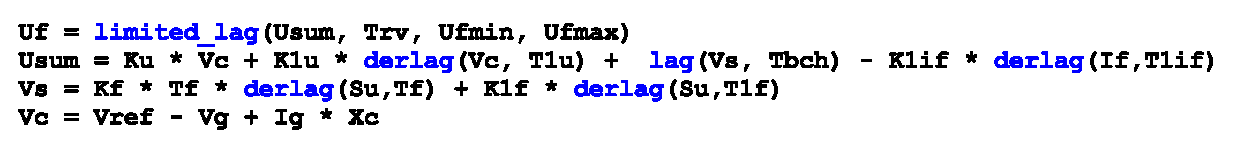
\includegraphics[width=\columnwidth]{code.eps}
	\caption{Sample AVR model pesudocode representation}
	\label{fig_avrcode}
\end{figure}
Textual form of representation is shown in Fig. \ref{fig_avrcode} and block diagram in Fig. \ref{fig_avr}.
\begin{figure}[h]
	\centering
	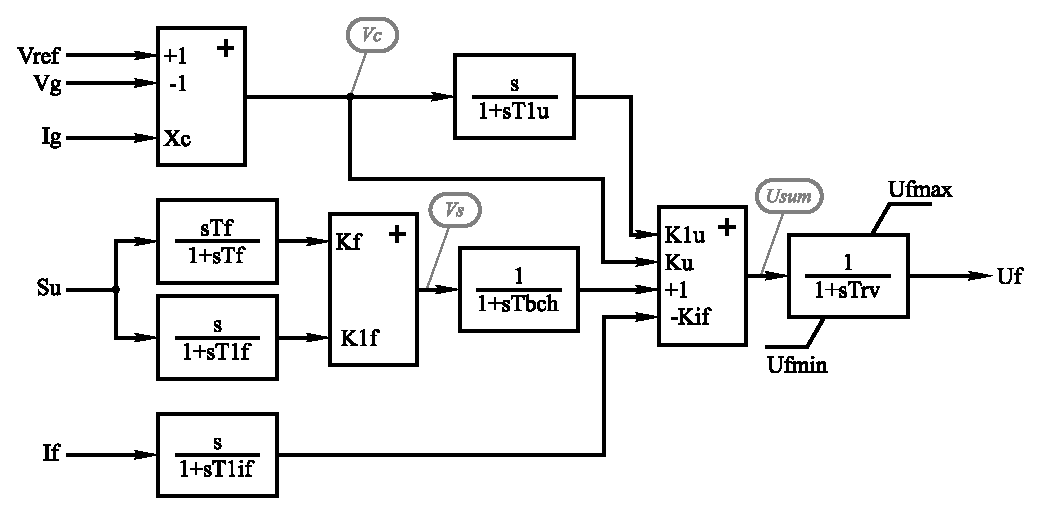
\includegraphics[width=\columnwidth]{avr.eps}
	\caption{Sample AVR model block diagram}
	\label{fig_avr}
\end{figure}

Both representations use elementary functional blocks: lag, derivative lag and limited lag. Ready-made elementary functional
blocks are included in custom model toolbox to simplify model creation and enable efficient implementation by software core 
instead of letting the user build these blocks from individual differential equations.
In addition, the implementation of the elementary blocks in the software core allows to use common procedures for discrete events 
location and processing and hide these details from the user. 
If necessary, differential equations can be explicitly specified using the integrator block.

Formally, the block diagram of the model corresponds to a directed graph whose vertices are elementary blocks, and
edges are defined by links. Compared to a conventional graph, the order in which the edges in a node are listed matters,
because elementary blocks have positional arguments that must be specified in a particular order. This imposes some restrictions
on the algorithms used in the implementation of custom models. The block diagram representation of custom models
turns out to be easier to use for implementation compared to textual one, since the order of calculations is readily
available by traversing graph from outputs to inputs, and validation of links and parameters is performed by the 
block diagram editor.

Creating a custom model in a text representation is reduced to describing a system of equations using generally accepted
mathematical operators and a set of built-in functions that also include elementary blocks. The system of equations must 
link the input and output variables. This provides for the possibility of using internal variables for structuring the 
system or introducing feedback. The description of the system is far from an intermediate language, so its transformation 
is required to implement the model. The textual representation is not as visual as the block diagram, 
but with some skill, it greatly speeds up the creation of models. At least text editors today remain the main means 
of professional software development and there is no trend towards the transition to graphical environments. 
It should be emphasized that the description of the model in the textual representation cannot be called a program in the
traditional sense of the term. The program sets the sequence of actions, while the solution sequence is not defined for th
e system of equations in textual representation. However, the implementation of the model must be nothing more than an ordinary
imperative program in the form of an executable module, therefore, in the process of transformations, 
the order of calculations must be determined.

To transform the custom model source data in text format, some general-purpose parsers are widely used. They are the programs
that allow to perform lexical and syntactic analysis of the source text according to a given dictionary and form the required 
data structure for further processing. Almost all programming languages use parsers in one way or another to generate 
intermediate object code from source code. Existing parsing technologies can also be used to analyze the textual representation 
of the model's system of equations. In the process of analyzing the original textual representation, the control of compliance 
with the specified rules and the detection of syntactic errors are performed. As a result of the analysis, a tree structure is
generated that allows performing the required transformations by manipulating the tree. To represent the system of equations 
of the custom model, a structure in the form of the abstract syntax tree (AST) is suitable. The nodes of such a tree are the
operators, and the edges define the mutual links of the operators. One of the possible options for converting the textual
representation of the AVR model from the example Fig. \ref{fig_avr}, \ref{fig_avrcode} into the AST is shown in Fig \ref{fig_ast}.

\begin{figure}[h]
	\centering
	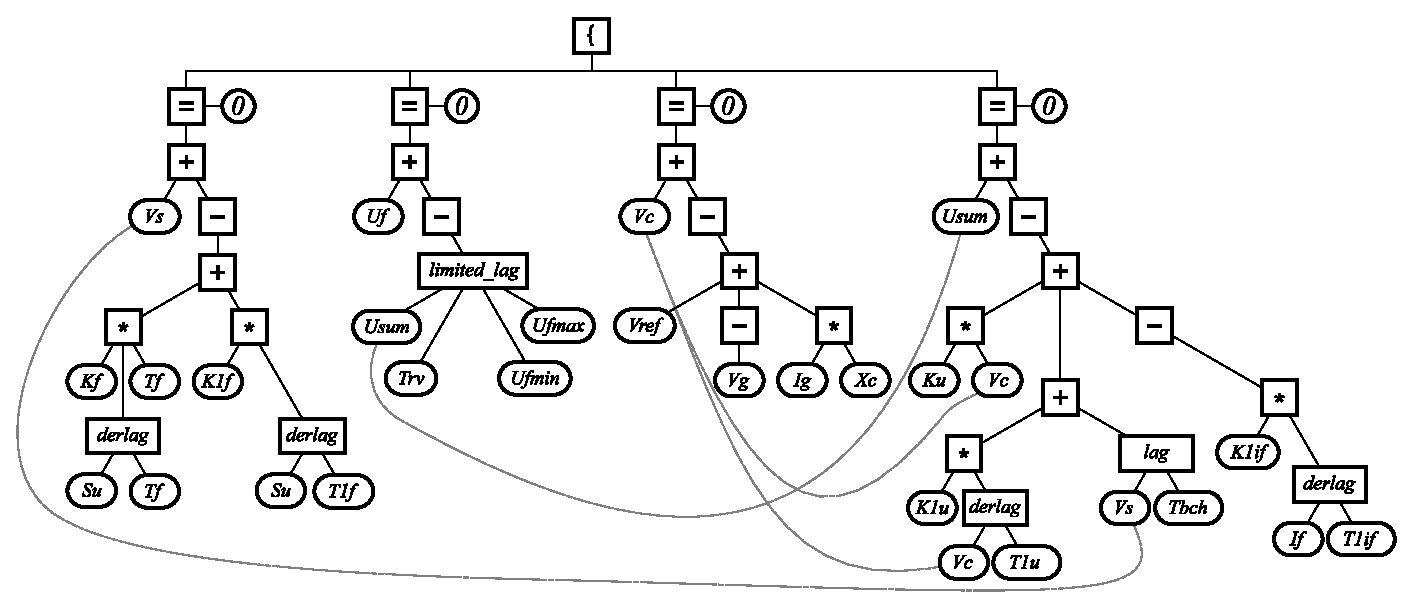
\includegraphics[width=\columnwidth]{ast.eps}
	\caption{Sample AVR model AST-tree }
	\label{fig_ast}
\end{figure}

In general, this structure is not a tree. The use of variables as operands of functional blocks turns the structure into a graph,
which, in the presence of feedbacks, cannot be reduced to the form of a tree. If there are several output variables, the structure
turns into a forest. The traditional use of the term "tree" is due to the fact that the structure is hierarchical and determines
the order of links of nodes. The AST shown in the Fig \ref{fig_ast}. Cycles on system variables are shown by dotted lines. 
If the edges of the connections of variables are not taken into account, then the graph can be considered directed from the lower
nodes to the upper ones. The edges of the variable connections do not have a given direction, but it can be determined 
provided if there are no feedbacks.

The root node of the tree marked as \raisebox{-2pt}[0pt][0pt]{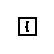
\includegraphics{eq.eps}} denotes a system of equations. 
Nodes marked as \raisebox{-2pt}[0pt][0pt]{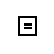
\includegraphics{let.eps}} represent individual equations. An equation node 
has two child nodes: a left a right. In AST, equations of the form \(f(x)=0\) are accepted, 
so if a non-zero expression appears on the right side in the process of transformation, it is transferred to the left 
side of the equation with a negative sign. Each equation node can resolve one of the model variables.

The form of AST for a given system of equations is not unique. For ASTs there is an identity rule, similar to the rule for
mathematical expressions. Two ASTs are identical if the values of the root nodes are equal on the entire set of values of the
variables included in them in their domains of definition. While maintaining identity, it is possible to perform AST 
transformations using subtree manipulations, achieving certain properties from the resulting AST. All manipulations of 
this kind are performed at the symbol level, that is, with variables whose values are unknown. Identity is preserved 
through the use of the rules of algebra and logic in the transformations. The AST structure is convenient for these 
transformations from an algorithmic point of view.

Taking as intermediate variables \(V_{c}\), \(V_{s}\) and \(U_{sum} \) at the figure points marked in the block diagram
of the model in Fig. \ref{fig_avr}, by traversing the graph from outputs to inputs, it is easy to obtain an AST 
identical to Fig. \ref{fig_ast}. One can also get the AST identical to shown in Fig. \ref{fig_ast} by transforming 
an arbitrary version of the AST built from block diagram. Thus, the AST can be used as an intermediate structure 
that is invariant with respect to the representation of the custom model. To build it, it is necessary to combine 
the analysis of the model graph with the analysis of text expressions. Due to this, the possibilities of describing 
the custom model in block diagram form can be significantly expanded. In particular, for the inputs and outputs 
of elementary blocks, mathematical expressions can be additionally specified in the textual representation. 
At the same time, the block diagram of the model remains compact and clear, and the user has almost unlimited 
possibilities for expanding the functionality of the model. The construction of an AST with such a combined approach 
begins with a traversal of the model graph, with a transition to the analysis of mathematical expressions. The results 
of parsing expressions are included in the graph AST as subtrees.

After transformation the representation of the model into the form of the AST, the main stage of the model implementation begins, which includes the following operations:
\begin{itemize}
	\item classification of variables;
	\item validation of the initial system of equations;
	\item simplification and optimization of mathematical expressions;
	\item generation of expressions for calculating partial derivatives;
	\item determination of the order of system of equations solution the by variables causalization.
\end{itemize}

\section{Custom model symbolic transformation}

\subsection{Model variables classification} \label{sec_varclass}
The block diagram or system of equations is the main, but not the only component of the source data for the implementation 
of the custom model. To link the model with software core, additional information is required, which, in particular, 
includes the declaration of variables. With the help of named variables, data exchange is arranged between 
the model and the software core, as well as with other models that are part of the system \eqref{eqn_thedae}. 
In addition to names, the declarations of variables includes attributes that allow them to be divided into classes according to
certain properties. The most important is the constant attribute. Variables with this attribute cannot be changed during the
simulation and are used to obtain source data when the model is initialized and the initial conditions are calculated. 
The attribute is also necessary for the correct formation of the system of model equations and determining the order of its solution. In the AST example above, the constants are variables for gains, time constants, and limits.

Variable attributes that explicitly define their properties must be specified in the model source data. But during the analysis
of the AST, some of the variables can receive the constant attribute implicitly. For example, an AST subtree in which only 
numerical values and constants act as variables is constant. If such an AST subtree resolves a state variable, then it will 
also be a constant. The definition of an implicit constant attribute affects the structure of the system of equations of the model.
Obviously, the number of equations must be equal to the number of unknown variables. Classification of one of the state variables 
as a constant requires eliminating one of the equations from the system. If the equality of the number of variables and 
equations is preserved, such an exception reduces the amount of calculations. However, in some cases, implicitly defining 
a variable as a constant may result in multiple equations being resolved, in which case the system becomes underdetermined. 
In such a situation, the model implementation process should terminate with an appropriate error message pointing the source data
problem.

Variables that are not classified as constants are state variables and, in turn, are divided into internal and external. 
Internal variables are resolved by model equations. External variables are references to internal variables of other models. 
In the example above, external to the AST model are the generator state variables \(S_u\), \(V_g\), \(I_g\), and \(I_f\) – 
rotor slip, terminal voltage, stator and rotor currents, respectively. In turn, the internal variable \(U_f\) will be interpreted as
external in the exciter model.

For state variables that are not constants, there is an intermediate class of discrete variables. It includes variables whose 
values can change only with discrete changes in the system of equations. These include, for example, variable output values of
logic elementary blocks. When the state of a logical block, the software core must perform the procedure for processing a
discontinuity in the system of equations by restarting the integration method with the calculation of new initial conditions,
including new values of discrete variables. In the time interval between discontinuities, the discrete variable has a constant
value. Thus, it makes no sense to include discrete variables into the system of model equations, considering their values in the
process of integration as constants. Calculation of the values of discrete variables is performed only when initialization and in
the discontinuity handling procedures. The definition of discrete variables is performed according to a principle similar 
to the implicit definition of constants: if the AST subtree resolves some variable and contains only constants and discrete
variables as, then the resolved variable is discrete.

\begin{figure}[h]
	\centering
	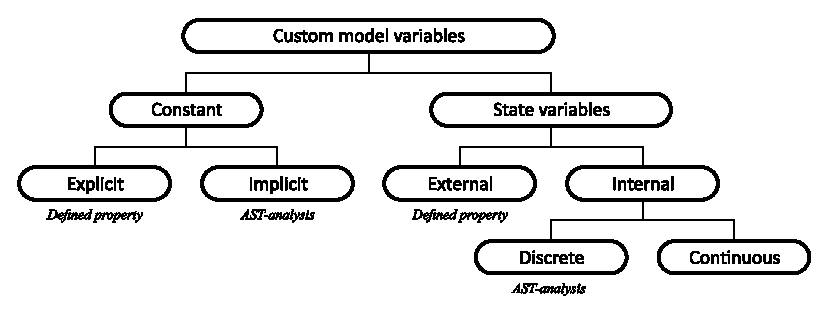
\includegraphics[width=\columnwidth]{variables.eps}
	\caption{Classification of the custom model variables}
	\label{fig_vars}
\end{figure}

State variables not classified as discrete or costant are ordinary continuous variables and are resolved by the system of model
equations as part of system \eqref{eqn_thedae}. The Fig. \ref{fig_vars} shows a simplified variables classification structure,
indicating how variables can be assigned to classes. 
It should be noted that the variables are not divided into differential and algebraic, which is due to the fact that the 
integration process in a particular implementation is based on the Gear method \cite{gear71}.

\subsection {Equation system source data validation} \label{sec_validation}

In the process of automatic custom model implementation, two phases of validation of the source data can be distinguished. 
The first phase is to detect errors that prevent the correct generation of the AST based on graphical or textual representations. 
In the graphical representation of the source data, a set of elementary blocks corresponding to the AST nodes is defined,
therefore, only topology validation is necessary: checks of unconnected inputs and outputs, the direction of connections from
outputs to inputs, etc. In order to prepare a text representation for generating an AST, it must be first parsed from the text 
and then checked or syntax errors, most of which prevent correct connections generation between AST nodes, and in some cases 
make it impossible to determine the set of AST nodes.

Once the AST has been generated, a second phase of validation can be performed, which is to detect semantic errors. The second phase
does not depend on the way the model is presented initially, since it uses only the AST and the results of the variables 
classification. This information allows validation of AST nodes that have received the constant attribute. In particular, 
the AST allows to ensure that those elementary block arguments that must be given as constants are defined by a constant subtrees. Since there are no restrictions on the structure of equations in text representation, it is possible for an equation to explicitly
or implicitly change the value of a variable with a constant attribute. Detection of this kind of errors can also be performed 
by the AST.

If the values of the child nodes of some AST node can be calculated from the given constants, it becomes possible to check 
the result of calculation for compliance with the acceptable node values in the process of model implementation. Such nodes 
include, for example, division, square root, inverse trigonometric functions, elementary blocks with restrictions. 
Error analysis in constant expressions, of course, does not guarantee that the model will behave correctly for any values 
of the source data, but allows to identify errors that do not depend on the source data and will inevitably arise during the simulation process.

\subsection {Simplification and optimization of mathematical expressions} \label{sec_simplification}

The possibility of representing mathematical expressions in a tree structure is widely used in computer algebra systems \cite{gathen13}. 
The purposes of such systems go far beyond the simplification of mathematical expressions and is mainly focused on solving problems in a symbolic way,
up to automated proof of theorems. Parts of the technology of identical transformations of expressions are in demand in optimizing systems for translating program
code, which can also include the considered system for models implementation. Expression simplification in computer algebra systems acts as a utility function 
and is designed to display results in a compact, generally accepted form. There is no universal definition of the result of the expression simplification, so at
least two options are considered: in the form of factorization (for example, \((a+b)(a-b)\) or in the form of a polynomial \((a ^ 2-b ^ 2)\). In the context of 
the considered application for the implementation of custom models, the term "simplification" takes on a clearer meaning and implies the calculation of the
expression with minimum computation cost. If each AST node is assigned a score of the cost of performing an operation, then the total cost of resolving the AST 
can be determined. The task of simplification is reduced to finding an identical AST with minimal total computation cost. Considering that the costs of 
the operation of multiplication, and even more so of raising to a power, are higher than for the operation of addition, for the difference of squares 
considered in the example above, the result of simplification will be \((a+b)(a-b)\).

Identity transformations of the AST are performed according to a certain set of rules \(r_i\) forming the set \(R\). The rule \(r_i\) is an identity, 
on the left side of which the AST of the original form specified, and on the right - the transformed AST. For example, the rule for the difference of squares has the form shown in Fig \ref{fig_simpl}.

\begin{figure}[h]
	\centering
	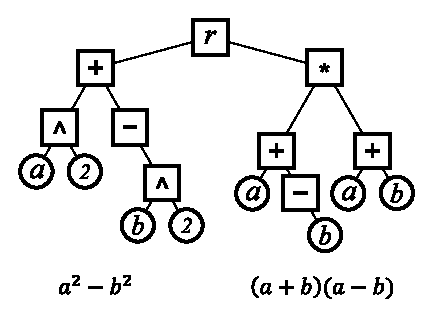
\includegraphics[width=.7\columnwidth]{simplification.eps}
	\caption{The difference of squares identity transformation rule}
	\label{fig_simpl}
\end{figure}

Since the rules define identities are reversible, they can be applied for transformations from the left AST to the right one and vice versa. 
In order to apply a rule, it is necessary to find in the source AST a subtree corresponding to the pattern of the AST of the part of the rule and replace it
with the AST subtree of the opposite part of the rule. At the same time, both when searching and when replacing, it must be taken into account that any subtrees 
of the original AST can act as arguments to the rules. In this example, these subtrees are labeled a and b. Thus, rules can be applied not only to 
expression variables, but to subexpressions.

Searching for a rule subtree pattern in the AST can be done recursively from top to bottom or bottom to top. For large ASTs, bottom-up search is more efficient, 
but it requires tree preprocessing. Since the AST changes during the application of the rules, the processing has to be repeated, therefore, 
the search for patterns is performed from top to bottom. When searching, one has to take into account permutations of arguments in nested 
AST nodes. For example, an addition operation with three terms yields 6 permutations, each of which must be checked against the pattern. 
In addition, some operations in AST are equivalent, such as exponentiation and successive multiplication. 
To reduce costs when searching for pattern rules, the AST is modified as follows:

\begin{enumerate}
	\item All commutative binary operators are replaced by n-ary ones. In this case, the subtree of consecutive binary operators of the same type is replaced by one operator node with \(n\) child nodes.
	\item Subtraction nodes are replaced by addition nodes with a unary minus.
	\item Division nodes are replaced by multiplication nodes. The divisor expression is enclosed in the exponentiation \(-1\).
	\item The child nodes are sorted in a certain order, which brings the AST to the so-called canonical form.
\end{enumerate}

Modifications 1, 2 and 3 eliminate the operations of subtraction and division and reduce the height of the AST, which simplifies the comparison of subtrees 
and reduces the required search depth. Modification 4 allows to eliminate the analysis of permutations when searching for rule patterns, since all child 
nodes will be in a defined order. Before generating the implementation of the model in the intermediate language, modifications 2 and 3 can be canceled by
converting to the original operations according to additional rules that are introduced into \(R\) at the final stage of system simplification.

To optimize the system of equations for performance, the set of rules \(R\) includes elementary rules of algebra (commutative, associative and distributive laws), 
rules of addition with zero and multiplication with zero and one, identities with powers, trigonometric and logarithmic identities. 
Since implicitly specified constants can be determined during the simplification process, the rules also include the calculation of AST nodes by numerical
arguments. If a numerical value of a node can be calculated, it is excluded from the AST together with the subtree and replaced with a numerical value. 
The total number of rules used is about fifty. All rules are represented in a special form of the AST.

A feature of the simplifications of the expressions used in this work is that they are performed for the entire system of equations, and not for
individual equations. Simplification algorithnm searches for repeated subexpressions, extacts them into a separate equation, and replaces the found
expressions with a variable using a substitution rule. Equations representation in canonical form \(f(x)=0\) eliminates the use of rules that must 
work on both sides of the equation, such as taking logarithms or exponentiation. In addition, this form of equations representation simplifies the
generation of expressions for partial derivatives and the determination of the order in which equations are solved.

Simplification and optimization of expressions in a system of equations consists in the sequential application of rules with the control of computational
cost reducing. The problem in what order and which rules to apply to achieve a minimum of costs does not have an unambiguous solution and in most cases
is solved by enumeration of possible variants. The solution of this problem is complicated by the fact that the sequence leading to the form of 
the system with minimal computational costs includes intermediate forms with higher costs than the original form. Therefore, when solving, it 
is not possible to use objective function indicating the optimal sequence. In addition, as in most problems of finding a global minimum, 
the solution can be achieved by exhaustive enumeration of all possible combinations, which is inapplicable in practice even for small systems and a
reduced set of rules. For the problem of simplification and optimization of the system of equations, two approaches were tested in this work. 
Both do not guarantee the achievement of a global minimum of costs, but can significantly reduce costs (if possible) for an acceptable time of
source data processing.

The first approach implies separation of \(R\) into two subsets: \(R_1\) and \(R_2\). The subset \(R_1\) includes the rules that generate the 
polynomial form of expressions, and \(R_2\) includes the rules for the factorized form. \(R_1\) and \(R_2\) are sequentially applied to the original 
system of equations until the computational cost stops decreasing. This approach is similar to that used with manual simplification of expressions. 
First, all the expressions are expanded by opening brackets, then they are factorized. This approach allows to reduce computational costs, mainly due to 
the fact that in the process of sequential application of \(R_1\) and \(R_2\), some of the AST nodes is converted into constants.

The second approach is more general and is based on finding a path in the graph \(G(F,T)\), where \(F\) are identical forms of the simplified system,
\(T\) are transformations performed according to the rules \(R\). \(A^*\) search algorithm \cite{pearl84} is used for path search. The original
algorithm is designed to find the shortest path between given nodes in a weighted graph and is used, for example, to build routes on flat maps. 
The difference from the equation system simplification problem is that the target node is not specified in the source data and must be determined 
by the minimum cost. A distinctive feature of \(A^*\) is that it preserves all paths from the source node to the destination. This allows to track
changes in costs and cut off paths where costs do not decrease. However, the time spent on its execution will be exponential.Ways to reduce
the cost of time is heuristic pruning of "dead end" paths and limiting the depth of paths to be searched

Practical studies show that in most cases the first approach allows to obtain an acceptable result. The second approach is used optionally, 
since it is more complex and not well determined, but in some cases it can significantly reduce computational costs compared to the original 
system due to the fact that it is able to “overcome” a sharp increase in computational costs at the initial stages of system 
simplification and determine the optimal order for applying the rules.

It should be noted that the purpose of simplification of the expressions of the user model is not only to reduce computational costs, but also to
additionally check the consistency of the given system. In the process of simplification, a situation may arise in which dependent equations are
eliminated, but the number of variables remains unchanged. Therefore, in the process of simplification, the consistency of the system is controlled
according to the rules given in subsection \ref{sec_validation}.

\subsection{Automatic differentiation}

At this stage of the implementation of the custom model, the system of equations is reduced to the final version with the minimal achieved
computational costs and prepared for linking with the software core. To solve the system of equations of the model, it is necessary to build 
a block of the matrix of partial derivatives. For models implemented by a software developer, this stage is performed manually according 
to a given system of equations. To implement a custom model, the generation of symbolic expressions for calculating partial 
derivatives must be fully automatic.

\begin{figure}[h]
	\centering
	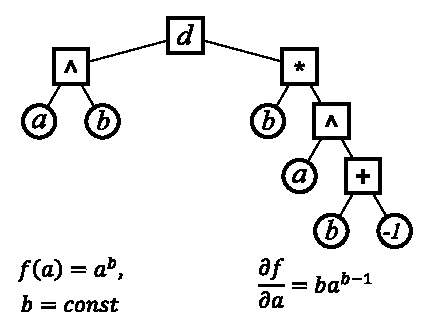
\includegraphics[width=.7\columnwidth]{derivative.eps}
	\caption{The power rule in form of AST}
	\label{fig_dpower}
\end{figure}

The problem of determining expressions for calculating partial derivatives is solved using symbolic manipulations using the system of equations AST.
Differentiation is performed analytically and eliminates the errors of numerical differentiation in transient simulations. 
The expressions for calculating partial derivatives is determined using template rules \(d_i\), which form a set of differentiation 
rules \(D\). The rules are defined for each type of AST nodes. As an example in Fig. \ref{fig_dpower} shows the rule for the partial 
derivative of the power function node.

If a differentiation rule is set for each of the types of AST nodes, then using a chain rule an ASD of a system of partial differential equations can be
obtained, in which each equation is assigned to an element of the Jacobi matrix of the custom model. Since the resulting expressions of partial 
derivatives will also be represented in the form of AST, the same simplification and optimization rules that were described in 
subsection \ref{sec_simplification} can be applied to them. The practical use of symbolic differentiation of functions has shown that a number of
expressions for partial derivatives turn out to be quite cumbersome and expressions can contain subexpressions that occur many times in the system. 
Simplification and optimization rules make it possible to detect such subexpressions and extract them into separate equations, which significantly
reduces the computational costs of calculating partial derivatives.

Since the optimization of expressions of partial derivatives is somehow carried out by introducing additional equations for repeated subexpressions,
a variant with a preliminary transformation of the model equations AST into the so-called operator tree was considered. In the operator tree, 
each original AST node is assigned an intermediate variable \(s_i\):
\begin{equation}
	\label{eqn_opthree}
	s_i=op_i(s,z)
\end{equation}
\noindent where:
\begin{description}
	\item  \(s\) is the intermediate variables vector;
	\item  \(z\) state variables vector;
	\item  \(op_i\) is the function defined by AST node;
\end{description}

There are no complicated functions in the operator tree, so only differentiation rules can be used to calculate partial derivatives with no need
to use chain rule.  The expressions obtained according to such rules are relatively compact and the computational costs for partial
derivatives, most often, turn out to be lower compared to optimized expressions for complicated functions. Of course, the reduction in 
computational costs is achieved by increasing the number of equations in the system. However, in this work, to solve the system of linear equations
with a matrix of partial derivatives, the matrix is transformed into a block triangular form \cite{davis12}. This form is constructed by  
permutation of the system so that non-zero values are located above diagonal, which in turn is free of zeros. 
After permutation, blocks remain on the diagonal, each of which, in the process of solving of the system, is subjected to LU decomposition 
with partial pivoting. The solution of the systems reduced to a back substitution in block form. Transformation of the AST into an operator form 
increases the dimension of the system being solved, but does not lead to the appearance of blocks on the diagonal, since all \(s_i\) are 
resolvable with respect to \(op_i\), and \eqref{eqn_opthree} can be interpreted not as an equality, but as an assignment. Thus, the addition 
of equations associated with the translation of the AST into an operator form is equivalent to the introduction of intermediate variables in the
calculation of partial derivatives, and its effect on the performance of the solution of the system is negligible.

The operator form of th AST also has a certain advantage, which allows for each operation in the system of equations of the custom model to 
obtain a result in he form of \(s_i (t_n)\) in the process of simulation. This feature is useful for in-depth analysis of the custom model 
in the process of its development and debugging. It should also be noted that the automatic differentiation tool provides significant support 
in the process of model development in the traditional way - by the software developer, as it eliminates the work of manual writing 
several tens or hundreds of expressions for partial derivatives.

\subsection{Determination of the order of the system of equations solution} 

There is no need to determine the order of solution for solving the system of equations of the custom model.
However, the overall performance of the simulation slightly affected by the pre-ordering of the system of
equations into a block triangular form. This reduces the cost of ordering of the complete system 
\eqref{eqn_thedae} in the software core. The question of the order of solution arises in the problem of
calculating the initial conditions at the points \(z_0 (t_0)\) and \(z_d (t_d)\). When the custom model is
implemented by the developer, the initial system is subjected to analysis, on the basis of which the 
procedure for determining the initial conditions for all elementary blocks and model variables is determined. 
If there are no feedbacks in the model, this order is reduced to a sequence of assignments, usually in the
direction from the output to the inputs. In the presence of feedbacks, the sequence requires the solution of
subsystems of equations, in general case, nonlinear ones. In most cases, the procedures for determining the
initial conditions at \(t_0\) and at \(t_d\) are the same. The only difference is that at \(t_0\) it is assumed:

\begin{equation}
	\label{eqn_opthree}
	\frac{df}{dt}(t_0)=\frac{dg}{dt}(t_0)=0,
\end{equation}

\noindent while for \(t_d \)this condition is not met, but the values of the derivatives at 
\(t_{d-}\) (up to the point of discontinuity) are known. Differential variables in most cases are considered continuous:

\begin{equation}
	\label{eqn_cont}
	\dot{y}(t_{d-})=\dot{y}(t_{d+}),
\end{equation}
\noindent which gives ability to resolve \(x(t_{d+})\).

The presence in the model of elements with integration constants, the values of which are determined using complicated logic,
significantly hampers calculation of the initial conditions. For example, the initialization of the PID controller or the
implementation of bumpless control according to this law, depending on the given coefficients, may require the rejection of 
\eqref{eqn_cont} and does not allow to determine the initial conditions in a general form \cite{fabozzi17}. In this case, 
it is required to supply extra source data of the custom model in the form of so-called initialization scheme, which explicitly
specifies expressions for determining the initial conditions.

In the simplest cases, when \eqref{eqn_thedae} does not contain nonlinear feedbacks and complicated logic that determines the
integration constants, the initialization scheme can be constructed automatically by analyzing the original system. 
Since the AST in operator form is used to solve this problem, a sufficient condition is the availability of the inverse 
function \(op^{inv}\) to the operator op, which allows resolving the variable from the equation of the AST node. 
The ability to solve an equation with respect to some variable is determined on the classification of variables described in
subsection \ref{sec_varclass} and the set of already resolved variables. To determine the order of equations resolving, 
an algorithm for finding the strongly connected components in the graph \(G(V,E)\), where \(V\) are state variables and \(E\) 
are equations, can be applied. One of the most efficient is Tarjan's algorithm \cite{sedgwwick11}.

If there are feedbacks in the original system, then ordering the equations in the form of a simple sequence of calculations
becomes impossible. Feedbacks form the so-called algebraic cycles, the solution of which requires the solution of a system of
equations. In this case, the ordering algorithm chooses the variable that allows the largest number of loop equations to be
resolved, and continues ordering the equations as if that variable were resolved. If there is an inverse function for the
equation of such a variable, the variable is introduced into the system of cycle equations using a substitution. 
This technique does not guarantee the solution of the system of equations, but will allow the system of equations to be 
ordered so that it acquires a block triangular form with diagonal blocks of the minimum size. Thus, the initial system, 
already in the process of implementation, takes on a form that does not require additional ordering in the software core.

In case the ordering algorithm copes with the task of resolving all variables, the custom model can be converted into an
intermediate language program. Otherwise, the algorithm produces a list of variables and equations that could not be resolved,
and the user must supply extra data of the model with the necessary initialization equations. The main reason that not all 
state variables can be resolved is the lack of inverse functions for AST nodes or functions used for variable substitutions. 
In this case, the simplest way to resolve a variable is to explicitly specify an expression to calculate its value in the 
initial conditions.

Improving the capabilities of algorithms for determining the initial conditions is the subject of further research. 
The presence of algebraic cycles in itself is not a problem, since they are solvable as a system of equations. The main 
problems in solving \eqref{eqn_thedae} at points \(t_0\) and \(t_d\) are related to the ambiguity in determining the 
integration constants and the states of logical elementary blocks. To obtain unique and feasible solution of the system, 
additional source data must be taken into account. One of the possible options is to provide ready-made implementations 
of complicated logical elements as elementary blocks. A more versatile approach implies addition of extra source data by 
extending model representation. Possible extension options are the use of Petri nets or finite state machines.

\section{Conclusion}

The process described above is implemented in a special compiler of the transient stability modeling package. The compiler accepts
model block diagram graph, textual description of the system of equations, or a mixed description consisting of
graph with additional equations for elementary blocks. The compiler supports more than 50 elementary blocks and allows
generate source code in an intermediate language for subsequent translation into native code. C++17 is used as an intermediate language. 
The result of compilation is a dynamic library with the implementation of the functions necessary for the model to interact with the software core. 
Using the compiler is not only a equipment model can be implemented, but also models of automatic devices and transient stability simulation scenarios.

The use of symbolic manipulations allows to fully automate the implementation of custom models
for transient stability simulation. In the process of implementing the model, symbolic manipulations make it possible
optimize models to improve performance and provide advanced error checking. The source data of custom models can be graphic
representation, textual representation, or a mix of both, which allows to combine the capabilities of different modeling
approaches without the need to involve software developers.

\begin{thebibliography}{1}
\bibliographystyle{IEEEtran}
\bibitem{sumulink}
Simulink - Simulation and Model-Based Design // www.mathworks.com. [2020]. URL: https://www.mathworks.com/products/simulink.html
\bibitem{modelica}
Modelica Language Documents - Version 3.4 - April 2017. // modelica.org. [2020]. URL: https://modelica.org/documents. 
\bibitem{eurostag}
Flexible and secure modeling // www.eurostag.be. URL: http://www.eurostag.be/en/products/eurostag/features/flexible-and-secure/flexible-secure/.
\bibitem{sincal}
PSS SINCAL Platform // www.simtec-gmbh.at. URL: http://www.simtec-gmbh.at/sites\_en/platform.asp.
\bibitem{powefactory}
Francisco Gonzalez-Longatt and Jos{\'{e}} Luis Rueda Torres. Advanced Smart Grid Functionalities Based on PowerFactory. Springer International Publishing AG, 2018.
\bibitem{gear71}
Gear C.W. The Simultaneous Numerical Solution Of Differential - Algebraic Equations SLAC-PUB-0723. // IEEE Trans.Circuits Theory, No. 18, 1971. pp. 85-95.
\bibitem{gathen13}
Joachim von zur Gathen, Jürgen Gerhard. Modern Computer Algebra. 3rd ed. Cambridge University Press, 2013.
\bibitem{pearl84}
Pearl J. Heuristics: Intelligent Search Strategies for Computer Problem Solving. Addison-Wesley Pub, 1984.
\bibitem{davis12}
Timothy A. Davis, E. Palamadai Natarajan. Sparse Matrix Methods for Circuit Simulation Problems // In: Scientific Computing in Electrical Engineering. Springer, Berlin, Heidelberg, 2012. pp. 3-14.
\bibitem{fabozzi17}
Davide Fabozzi, Stefan Weigel, Bernd Weise, Fortunato Villella. Semi-implicit Formulation of Proportional-integral Controller Block with Non-windup Limiter According to IEEE Standard 421.5-2016 // Proceedings Of IREP'2017 Symposium, 2017.
\bibitem{sedgwwick11}
Robert Sedgewick, Kevin Wayne.  Algorithms. 4th ed. Pearson Education, 2011.
\end{thebibliography}

\newpage
\section{Biography Section}
\vspace{-33pt}
\begin{IEEEbiography}[{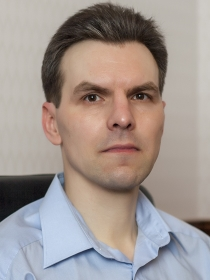
\includegraphics[width=1in,height=1.25in,clip,keepaspectratio]{mashalov}}]{Eugene Mashalov}
Graduated from Electrotechnical Faculty, Ekaterinburg, Urals State Polytechnical University, 1997. 
Received Ph.D degree in 2000 from the same university. 
Works for JSC "Scientific and Technical Center of Unified Power System", Ekaterinburg, Russia.\\
mashalov@gmail.com \\
www.inorxl.com
\end{IEEEbiography}
\vfill
\end{document}


